% !TeX spellcheck = es_ES
\documentclass[12pt, titlepage]{article}
\usepackage[utf8]{inputenc}
\usepackage[spanish]{babel}
\usepackage{float}
\usepackage[letterpaper, margin=2.5cm]{geometry}
\usepackage[nottoc,notlot,notlof]{tocbibind} % Hace que se agregen las referencias al indice
\usepackage{url}
\usepackage{graphicx} 
\usepackage{listings}
\usepackage{color}
\definecolor{dkgreen}{rgb}{0,0.6,0}
\definecolor{gray}{rgb}{0.5,0.5,0.5}
\definecolor{mauve}{RGB}{253,151,31}

\lstset{frame=tb,
    language=Sql,
    aboveskip=3mm,
    belowskip=3mm,
    showstringspaces=false,
    columns=flexible,
    basicstyle={\small\ttfamily},
    numbers=none,
    numberstyle=\tiny\color{gray},
    keywordstyle=\color{blue},
    commentstyle=\color{dkgreen},
    stringstyle=\color{mauve},
    breaklines=true,
    breakatwhitespace=true,
    tabsize=2,
    morekeywords={use}
}

\title{Reporte: Práctica 3}
\author{Carlos Tonatihu Barrera Pérez \\ Profesor: Hernández Contreras Euler \\ Bases de Datos \\ Grupo: 2CM1 }
\date{3 de marzo de 2017}

\begin{document}
    \maketitle
    \tableofcontents
    \section{Marco Teórico}
    El lenguaje de definición de datos SQL (el cual es usado para realizar estas practicas) se utiliza para crear relaciones con esquemas especificados.
    SQL cuenta con tres principales clausulas a la hora de hacer consultas:
    \begin{itemize}
    \item La clausula \textbf{select} se corresponde con la operación de proyección del álgebra relacional. Se usa para obtener una relación de los atributos deseados en el resultado de una consulta.
    \item La clausula \textbf{from} se corresponde con la operación producto cartesiano del álgebra relacional. Genera una lista de las relaciones que deben ser analizadas en la evaluación de la expresión
    \item La clausula \textbf{where} se corresponde con el predicado selección del álgebra relacional. Es un predicado que engloba a los atributos de las relaciones que aparecen en la clausula \textbf{from}.
    \end{itemize}
    \begin{figure}[H]
        \begin{center}
            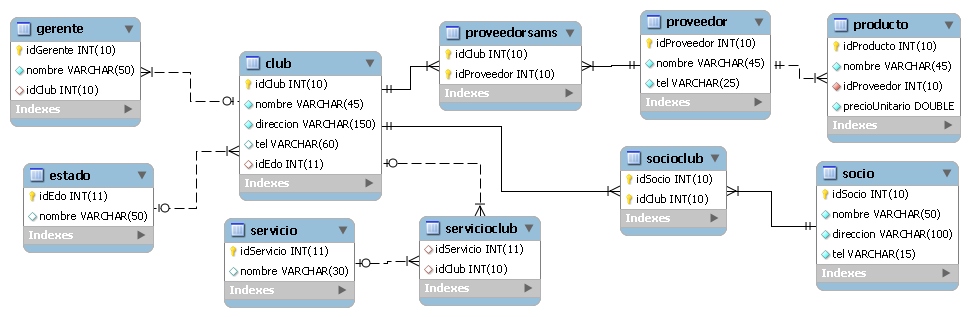
\includegraphics[width=12cm, height=6cm]{img/sams.png}
            \caption{Script usado.}
            \label{fig:hasta-use}
        \end{center}
    \end{figure}
    \newpage
    \section{Desarrollo}
        En esta practica se trabajo con un script llamado sams.sql por lo que se creo una base de datos para trabajar y despues se importo el contenido del script.
        \begin{figure}[H]
            \begin{center}
                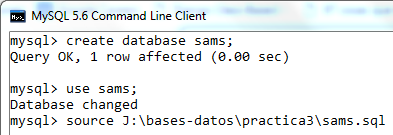
\includegraphics[width=12cm, height=6cm]{img/source.png}
                \caption{Creación y uso de la base.}
                \label{fig:hasta-use}
            \end{center}
        \end{figure}
        \begin{figure}[H]
            \begin{center}
                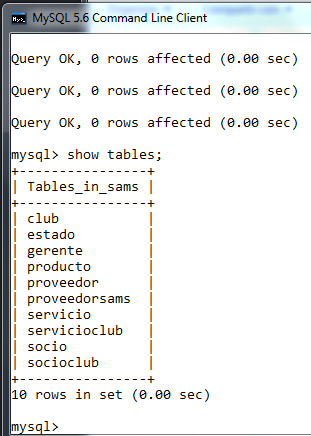
\includegraphics[width=16cm, height=10cm]{img/post-source.png}
                \caption{Resultado de ejecutar el source.}
                \label{fig:tablas}
            \end{center}
        \end{figure}
    Ahora comenzamos con el uso del comando select, debido a que lo que despliegan las tablas son demasiados datos en las imágenes solo se muestran los primeros resultados.
    \begin{figure}[H]
        \begin{center}
            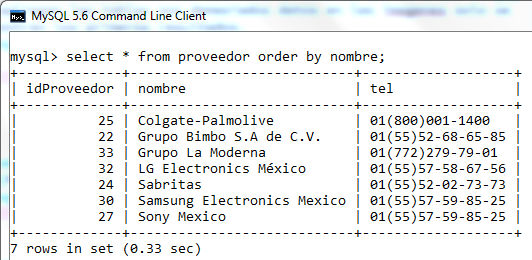
\includegraphics[width=10cm, height=11cm]{img/campos.png}
            \caption{Se muestran todos los campos y se ordena por nombre el contenido de proveedor.}
            \label{fig:arlter}
        \end{center}
    \end{figure}
\begin{figure}[H]
    \begin{center}
        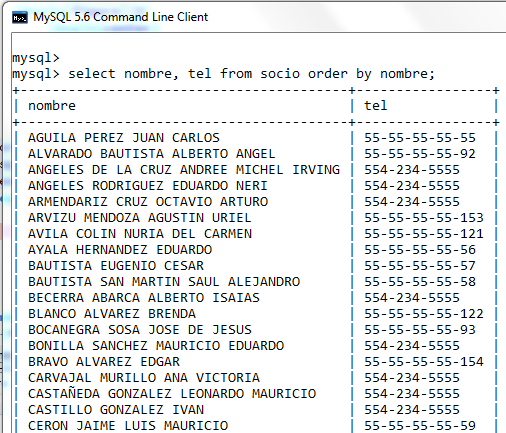
\includegraphics[width=10cm, height=11cm]{img/order.png}
        \caption{Muestra algunos campos y se ordenan por nombre.}
        \label{fig:arlter2}
    \end{center}
\end{figure}
\begin{figure}[H]
    \begin{center}
        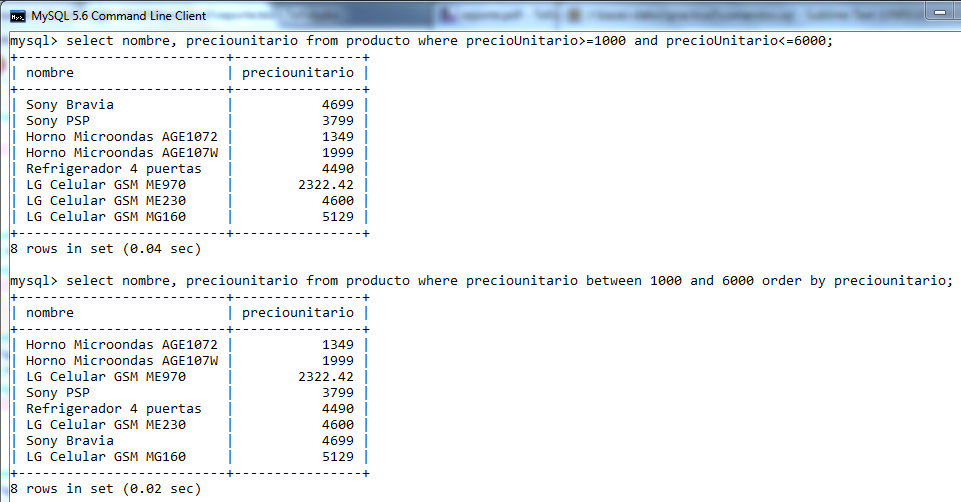
\includegraphics[width=10cm, height=11cm]{img/entre.png}
        \caption{Desplegamos los campos con un precio unitario entre 1000 y 6000 de dos formas distintas.}
        \label{fig:arlter3}
    \end{center}
\end{figure}
\begin{figure}[H]
    \begin{center}
        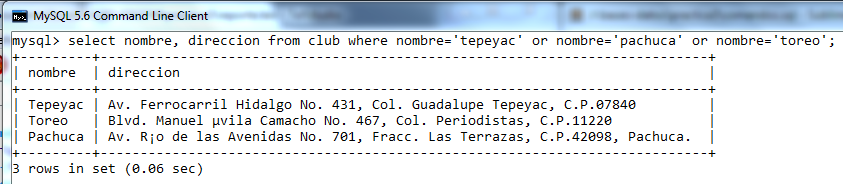
\includegraphics[width=10cm, height=11cm]{img/club.png}
        \caption{Información de los club con los nombres de tepeyac, toreo o pachuca.}
        \label{fig:arlter4}
    \end{center}
\end{figure}
\begin{figure}[H]
    \begin{center}
        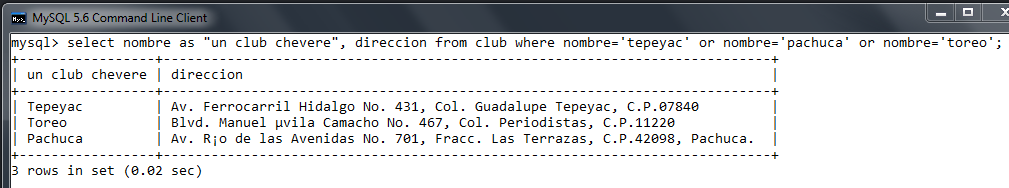
\includegraphics[width=10cm, height=11cm]{img/chevere.png}
        \caption{Lo mismo que el anterior pero renombrando la columna nombre como "un club chevere".}
        \label{fig:arlter5}
    \end{center}
\end{figure}
En este punto se empezo a usar la palabra reservada 'like' que es una wildcard (comodín) para las consultas un poco más complejas.
\begin{figure}[H]
    \begin{center}
        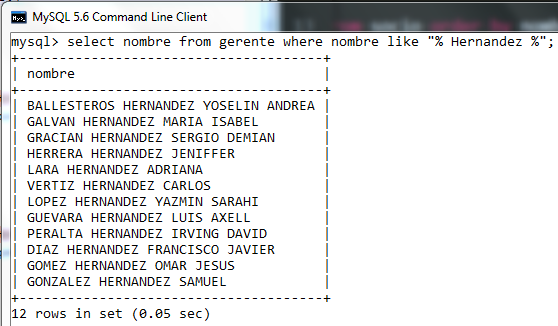
\includegraphics[width=10cm, height=11cm]{img/hernandez.png}
        \caption{Mostramos a todos aquellos que se apelliden Hernandez.}
        \label{fig:arlterotro}
    \end{center}
\end{figure}
\begin{figure}[H]
    \begin{center}
        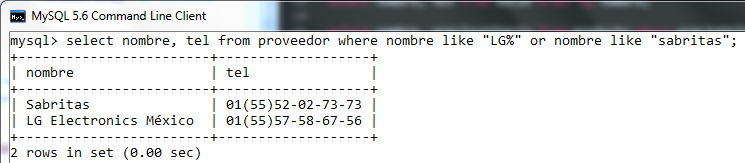
\includegraphics[width=10cm, height=11cm]{img/sabritas.png}
        \caption{Se muestran todos los teléfonos de los proveedores de LG y sabritas.}
        \label{fig:arlter6}
    \end{center}
\end{figure}
\begin{figure}[H]
    \begin{center}
        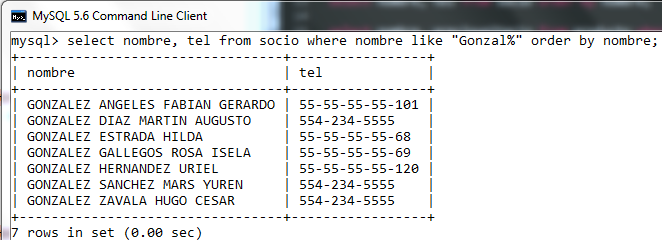
\includegraphics[width=10cm, height=11cm]{img/gonzalez.png}
        \caption{Muestra a aquellos socios con apellido paterno Gonzáles.}
        \label{fig:arlter7}
    \end{center}
\end{figure}
\begin{figure}[H]
    \begin{center}
        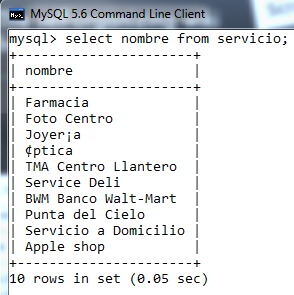
\includegraphics[width=10cm, height=11cm]{img/servicios.png}
        \caption{Muestra el nombre de todos los servicios disponibles.}
        \label{fig:arlter8}
    \end{center}
\end{figure}
\begin{figure}[H]
    \begin{center}
        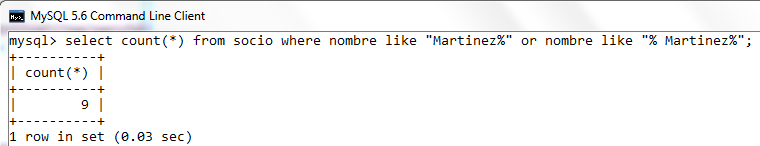
\includegraphics[width=10cm, height=11cm]{img/martinez.png}
        \caption{Cuenta cuantos socios se apellidan Martínez.}
        \label{fig:arlter9}
    \end{center}
\end{figure}
\begin{figure}[H]
    \begin{center}
        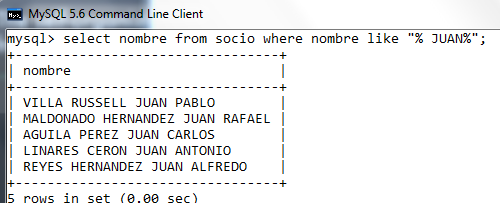
\includegraphics[width=10cm, height=11cm]{img/juan.png}
        \caption{Muestra el nombre de los socios llamados Juan.}
        \label{fig:arlter10}
    \end{center}
\end{figure}
Después de hacer algunas consultas comenzamos a modificar las relaciones comenzando renombrar la tabla gerente.
\begin{figure}[H]
    \begin{center}
        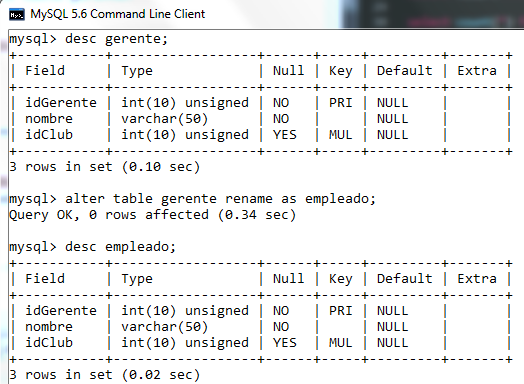
\includegraphics[width=10cm, height=11cm]{img/nombre.png}
        \caption{Cambio nombre.}
        \label{fig:arlter77}
    \end{center}
\end{figure}
Se hicieron cambios en la tabla estado.
\begin{figure}[H]
    \begin{center}
        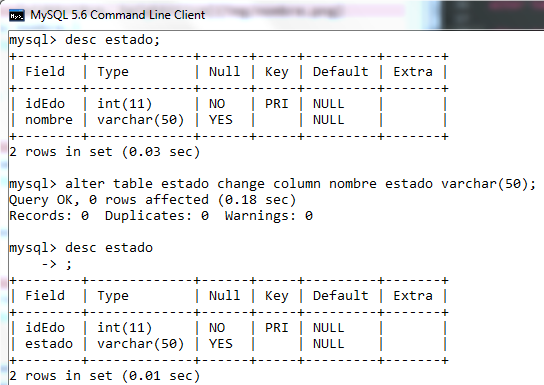
\includegraphics[width=10cm, height=11cm]{img/change.png}
        \caption{Cambiamos el nombre del campo nombre a estado.}
        \label{fig:arlter90}
    \end{center}
\end{figure}
De la misma forma se modifico la relación socio.
\begin{figure}[H]
    \begin{center}
        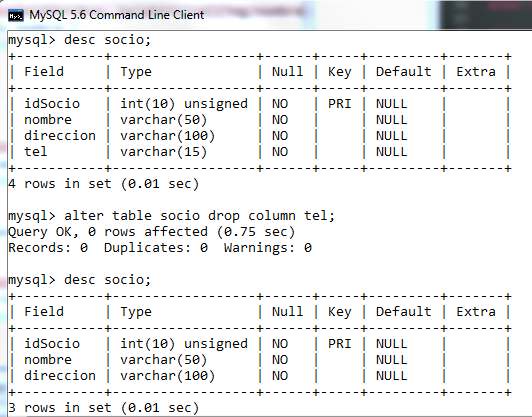
\includegraphics[width=10cm, height=11cm]{img/socio.png}
        \caption{Se elimino la columna tel y su contenido de socio.}
        \label{fig:arlter777}
    \end{center}
\end{figure}
A continuación se procedió a eliminar la llave foranea de la tabla producto.
\begin{figure}[H]
    \begin{center}
        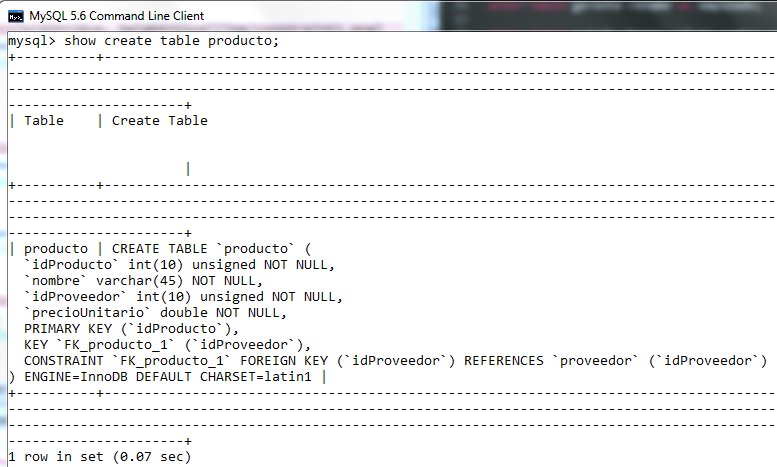
\includegraphics[width=10cm, height=11cm]{img/constraint1.png}
        \caption{Buscamos el constraint.}
        \label{fig:arlter11}
    \end{center}
\end{figure}
\begin{figure}[H]
    \begin{center}
        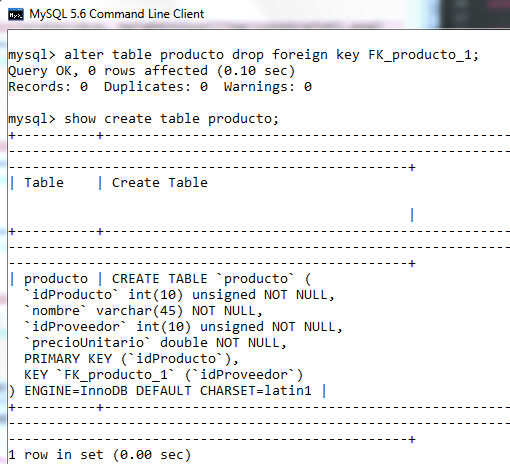
\includegraphics[width=10cm, height=11cm]{img/constraint2.png}
        \caption{Borramos la relación.}
        \label{fig:arlter12}
    \end{center}
\end{figure}
Creamos una llave primaria compuesta para empleado para hacer esto primero se elimina la llave primaria anterior.
\begin{figure}[H]
    \begin{center}
        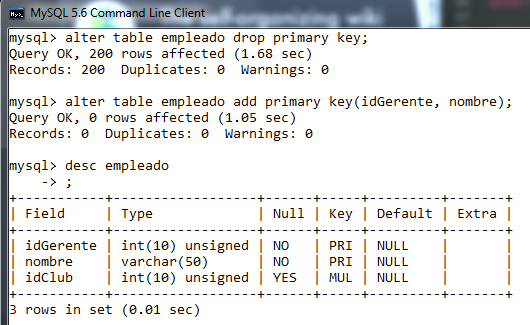
\includegraphics[width=10cm, height=11cm]{img/llave.png}
        \caption{Nueva llave primaria.}
        \label{fig:arlter13}
    \end{center}
\end{figure}
Luego se agrego el campo el campo salario de tipo double a la tabla empleado.
\begin{figure}[H]
    \begin{center}
        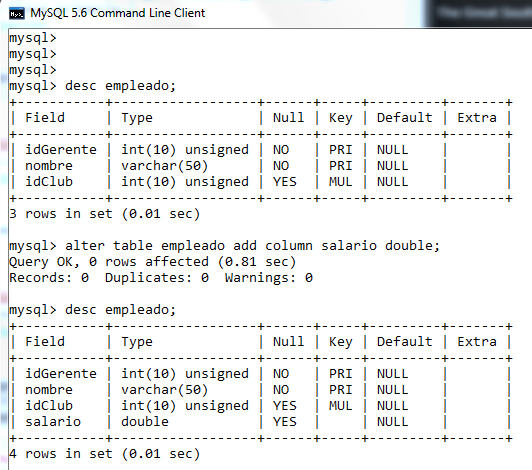
\includegraphics[width=10cm, height=11cm]{img/salario.png}
        \caption{Nueva descripción de la relación empleado.}
        \label{fig:arlter14}
    \end{center}
\end{figure}
Finalmente agregamos una nueva relación para poder manejar múltiples correos del socio.
\begin{figure}[H]
    \begin{center}
        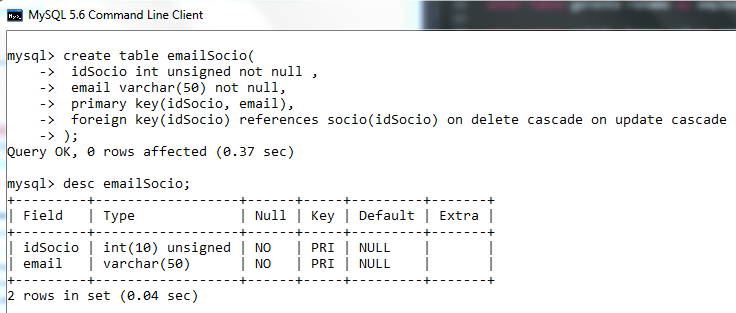
\includegraphics[width=10cm, height=11cm]{img/email-socio.png}
        \caption{Creación de la nueva tabla emailSocio.}
        \label{fig:arlter15}
    \end{center}
\end{figure}
    \section{Conclusiones}
        En esta practica se observo de una manera muy simple el funcionamiento de algunos comandos y diversas opciones que tienen para desplegar el contenido de las tablas lo cual en un futuro nos brindara las herramientas necesarias para buscar información y darle más funcionamiento a las aplicaciones que realicemos en el futuro.
    \bibliography{bibliografia} 
    \bibliographystyle{ieeetr}
\end{document}